%% LyX 2.3.6.1 created this file.  For more info, see http://www.lyx.org/.
%% Do not edit unless you really know what you are doing.
\documentclass[english]{article}
\usepackage[T1]{fontenc}
\usepackage[latin9]{inputenc}
\usepackage{geometry}
\geometry{verbose,tmargin=2.5cm,bmargin=2.5cm,lmargin=2.5cm,rmargin=2.5cm}
\usepackage{array}
\usepackage{calc}
\usepackage{textcomp}
\usepackage{multirow}
\usepackage{graphicx}
\PassOptionsToPackage{normalem}{ulem}
\usepackage{ulem}

\makeatletter

%%%%%%%%%%%%%%%%%%%%%%%%%%%%%% LyX specific LaTeX commands.
%% Because html converters don't know tabularnewline
\providecommand{\tabularnewline}{\\}

\makeatother

\usepackage{babel}
\begin{document}
{[}SPLIT\_HERE{]}
\begin{enumerate}
\item \textbf{{[}HCI/PRELIM/9569/2021/P1/Q1{]} }

An E-Commerce company stores the following data of customers in the
system. 
\begin{itemize}
\item Name 
\item Contact 
\item Address 
\end{itemize}
It categories its customers into 2 types of loyalty programs. 
\begin{itemize}
\item Spend-based loyalty program 
\item Paid loyalty program 
\end{itemize}
Customers of Spend-based loyalty program earn one point for every
block of \$10 spent in a single order, whereas customers of Paid loyalty
program pay a monthly or annual fee. Customers of Paid loyalty program
will enjoy the benefits of having early access to sales events and
free delivery for purchases above \$30. 

For Spend-based loyalty program, the additional data stored include: 
\begin{itemize}
\item Points earned 
\end{itemize}
For Paid loyalty program, the additional data stored include: 
\begin{itemize}
\item Payment schedule (monthly or annually) and corresponding fee 
\item Next payment date, computed based on payment schedule and the date
of enrollment to the program 
\end{itemize}
Object-oriented programming will be used to model the customers. 
\begin{enumerate}
\item Draw a class diagram that shows the following for the requirement
described above.
\begin{itemize}
\item the superclass 
\item any subclasses 
\item inheritance 
\item properties 
\item appropriate methods \hfill{}{[}6{]}
\end{itemize}
\end{enumerate}
The company makes changes to the Paid loyalty program to allow the
customer in the program to earn ten points for every block of \$20
spent in a single order, in addition to the current benefits. The
points earned do not expire. For Spend- based loyalty program, all
points earned will expire on the anniversary of the date of enrolment
to the program. 
\begin{enumerate}
\item[(b)]  Suggest changes required to the class diagram to enable the changes.\hfill{}
{[}3{]}
\item[(c)]  Explain why inheritance is an important feature of object-oriented
programming.\hfill{} {[}1{]}
\end{enumerate}
To attract customers to enrol to its Paid loyalty program, the company
launches an invitation campaign to invite Spend-based loyalty program
customers who qualified the following conditions: 
\begin{itemize}
\item Customer who earned more than 2000 points in a year and has an average
of at least one order per month will be contacted by staff. 
\item Customer who has enrolled for at least a year and has an average of
at least one order per month will be sent an invitation email. 
\item Otherwise, no invitation will be sent. 
\end{itemize}
\begin{enumerate}
\item[(d)]  Create a decision table showing all the possible outcomes and results.
\hfill{}{[}4{]}
\item[(e)]  Simplify your decision table by removing redundancies.\hfill{}
{[}2{]}
\end{enumerate}
{[}SPLIT\_HERE{]}
\item \textbf{{[}HCI/PRELIM/9569/2021/P1/Q2{]}}

Merge Sort is a Divide and Conquer algorithm. It divides the unsorted
array \texttt{A{[}low..high{]}} into two halves, calls itself for
the two halves, until each half is of length 1. It then merges the
two sorted halves. An algorithm for Merge Sort is given below. 

\noindent %
\noindent\begin{minipage}[t]{1\columnwidth}%
\texttt{PROCEDURE MergeSort(A, low, high) }

\texttt{\qquad{}IF low < high }

\texttt{\qquad{}\qquad{}mid \textleftarrow{} (low + high) DIV 2 }

\texttt{\qquad{}\qquad{}MergeSort(A, low, mid) }

\texttt{\qquad{}\qquad{}MergeSort(A, mid+1, high) }

\texttt{\qquad{}\qquad{}Merge(A, low, mid, high) }

\texttt{\qquad{}ENDIF }

\texttt{ENDPROCEDURE }%
\end{minipage}
\begin{enumerate}
\item Write in \textbf{pseudocode}, an algorithm for the merge procedure,
\texttt{Merge(A, low, mid, high)} that is called by the \texttt{MergeSort}
algorithm. The merge procedure should merge the sorted subarrays in
\texttt{A{[}low..mid{]}} and \texttt{A{[}mid+1..high{]}} into a single
sorted subarray in \texttt{A{[}low..high{]}}. \hfill{}{[}6{]}
\item Give and justify the time complexity of Merge Sort. \hfill{}{[}2{]}
\end{enumerate}
{[}SPLIT\_HERE{]}
\item \textbf{{[}HCI/PRELIM/9569/2021/P1/Q3{]}}

An abstract Data Type (ADT) consists of both data type and associated
operations. 

A stack ADT has the following operations defined: 
\begin{itemize}
\item Create(S) -{}-{}- creates an empty stack S, 
\item Insert(S, Item) -{}-{}- inserts new value, Item, onto stack S, 
\item Retrieve(S) -{}-{}- removes and returns item from the stack S, 
\item EmptyStack(S) -{}-{}- returns true if stack S is empty. 
\end{itemize}
\begin{enumerate}
\item Devise an algorithm that converts a non-negative integer from decimal
to hexadecimal, by making use of the stack operations given above.
\hfill{}{[}4{]}
\item Three items, L1, L2 and L3, are to be inserted into a stack in its
original order, but the output would be in the order of L1, L3 and
L2. 

Write an algorithm, using the operations given above, that would use
a stack R to carry this out. \hfill{}{[}4{]}
\end{enumerate}
{[}SPLIT\_HERE{]}
\item \textbf{{[}HCI/PRELIM/9569/2021/P1/Q4{]}}

Some algorithms can be written using recursion.
\begin{enumerate}
\item State \textbf{two} features of recursion. \hfill{}{[}2{]}
\item Explain the use of a stack when the recursive procedure executes.
\hfill{}{[}3{]}
\item Write a recursive function using \textbf{pseudocode} that returns
the sum of the digits in an integer. For example, the sum of the digits
of the integer \texttt{12345} is \texttt{5+4+3+2+1=15}. \hfill{}{[}4{]}
\end{enumerate}
{[}SPLIT\_HERE{]}
\item \textbf{{[}HCI/PRELIM/9569/2021/P1/Q5{]}}
\begin{enumerate}
\item Vaccination centres are located across the island to facilitate the
national vaccination programme. At each vaccination centre, data is
uploaded to the central system of Ministry of Health. 
\begin{enumerate}
\item State the name of this network structure. Describe \textbf{on}e disadvantage
and suggest \textbf{one} method to resolve it. \hfill{}{[}3{]}
\item Describe \textbf{two} rules of conduct for the staff handling data.
\hfill{}{[}2{]}
\end{enumerate}
\item Explain each of the following terms and how it works: 
\begin{enumerate}
\item Digital signature \hfill{}{[}7{]}
\item Transmission Control Protocol \hfill{}{[}3{]}
\item Domain Name System\hfill{} {[}2{]}
\end{enumerate}
\end{enumerate}
{[}SPLIT\_HERE{]}
\item \textbf{{[}HCI/PRELIM/9569/2021/P1/Q6{]}}

Check digit is one technique of data validation. 
\begin{enumerate}
\item[(i)]  Give \textbf{two} other techniques of data validation.\hfill{}
{[}2{]}
\item[(ii)]  With \textbf{one} example of data verification, explain the difference
between data verification and data validation. \hfill{}{[}3{]}
\end{enumerate}
A student ID consists of 5 digits and a check digit. 
\begin{enumerate}
\item[(iii)]  One way to calculate the check digit is to use the unit\textquoteright s
digit of the sum of all 5 digits. For example, suppose the 5 digits
are 50879. Since 5 + 0 + 8 + 7 + 9 = 29, the check digit is 9, and
the student ID is 508799. 

Explain, with \textbf{two} examples, why this method is inadequate.
\hfill{}{[}2{]}
\end{enumerate}
The check digit is calculated from the 5 digits using the modulus
11 system. It can be digits \texttt{0 - 9 }or character \texttt{'X'}. 
\begin{enumerate}
\item[(iv)]  Showing your working, determine the check digit for 30526. \hfill{}{[}3{]}
\item[(v)]  Write an algorithm to check if a student ID is valid. \hfill{}{[}5{]}
\item[(vi)]  A function is designed to read a student ID and determine if it
is valid. State the data types of its input parameter and justify.
\hfill{}{[}2{]}
\end{enumerate}
{[}SPLIT\_HERE{]}
\item \textbf{{[}HCI/PRELIM/9569/2021/P1/Q7{]}}
\begin{enumerate}
\item {}
\begin{enumerate}
\item What is a flowchart? \hfill{}{[}1{]}
\item Draw a flowchart to find the factorial of a given positive integer
\texttt{N}.\hfill{} {[}2{]}
\end{enumerate}
\item You have a row of \texttt{2}n disks of two colors, \texttt{n} black
and \texttt{n} white. They alternate: black, white, black, white,
and so on. You want to get all the black disks to the right-hand end,
and all the white disks to the left-hand end. The only moves you are
allowed to make are those that interchange the positions of two neighboring
disks.
\begin{center}

\includegraphics[width=0.5\paperwidth]{C:/Users/Admin/Desktop/Github/question_bank/LyX/static/img/9569-HCI-2021-P1-Q7}
\par\end{center}

Assume that there is an array \texttt{A} of size \texttt{2n} representing
the alternating disks. Write, in \textbf{pseudocode}, an algorithm
to solve this puzzle and determine the number of moves it takes. \hfill{}{[}5{]}
\end{enumerate}
{[}SPLIT\_HERE{]}
\item \textbf{{[}HCI/PRELIM/9569/2021/P1/Q8{]}}

The school is designing a website to allow ordering of meal. The database
stores data about 
\begin{itemize}
\item students 
\item meal information
\item order information 
\end{itemize}
An order contains one meal only. 

Each meal can be purchased by different students. 

A student never places more than one meal on any day. 

The data is stored in a relational database. 
\begin{center}
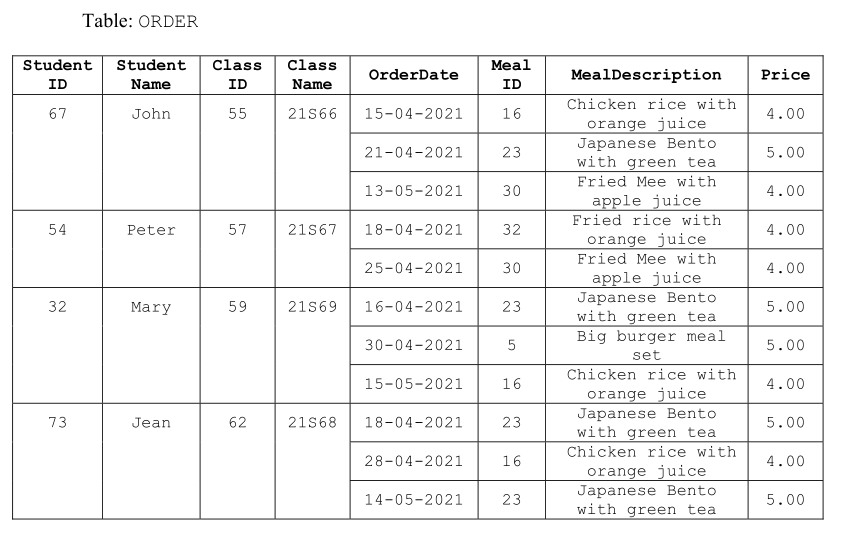
\includegraphics[width=0.5\paperwidth]{C:/Users/Admin/Desktop/Github/question_bank/LyX/static/img/9569-HCI-2021-P1-Q8-1}
\par\end{center}
\begin{enumerate}
\item Explain why the table is not in first normal form (1NF). \hfill{}{[}1{]}
\end{enumerate}
The following is an attempt to reduce data redundancy:
\begin{center}
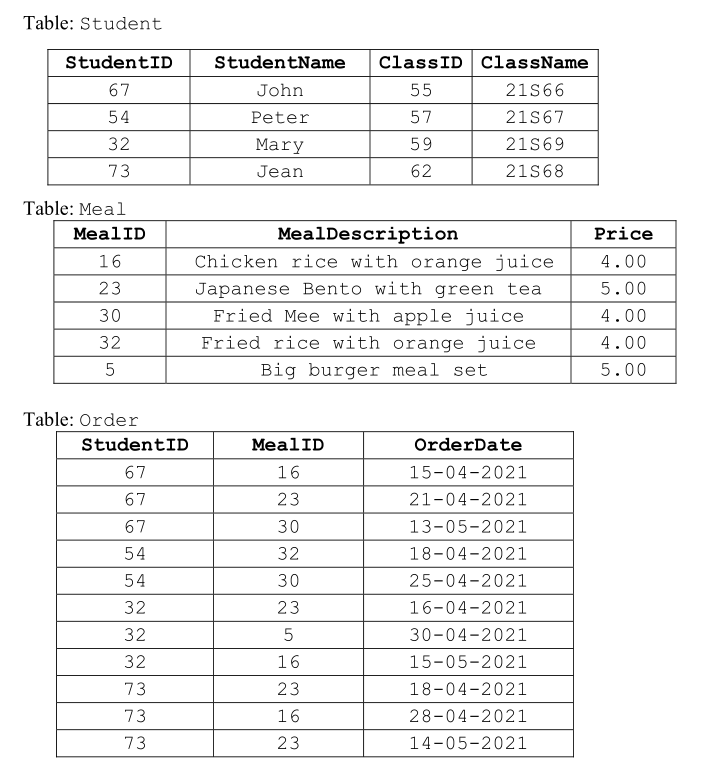
\includegraphics[width=0.5\paperwidth]{C:/Users/Admin/Desktop/Github/question_bank/LyX/static/img/9569-HCI-2021-P1-Q8-2}
\par\end{center}
\begin{enumerate}
\item[(b)]  State suitable primary key(s) for each table.\hfill{} {[}3{]}
\item[(c)]  Explain the reasons for reducing data redundancy in a relational
database. \hfill{}{[}2{]}
\item[(d)]  Draw an entity-relationship (E-R) diagram showing the degree of
the relations. \hfill{}{[}2{]}
\item[(e)]  State which table is not in third normal form (3NF) and explain
why. {[}2{]} 
\end{enumerate}
A table description can be expressed as: 
\noindent \begin{center}
\texttt{TableName (}\texttt{\uline{Attribute1}}\texttt{, Attribute2{*},
Attribute3, \dots ) }
\par\end{center}

The primary key is indicated by underlining one or more attributes.
Foreign keys are indicated by using a dashed underline/asterisk.
\begin{enumerate}
\item[(f)]  Write table descriptions for the required tables in the databases
so they are in third normal form (3NF). \hfill{}{[}4{]}
\item[(g)]  Write an SQL query to output the student names and date of order
of all the orders for the meal \textquotedblleft \texttt{Japanese
Bento with green tea}\textquotedblright .\hfill{} {[}3{]}
\end{enumerate}
{[}SPLIT\_HERE{]}
\item \textbf{{[}HCI/PRELIM/9569/2021/P2/Q1{]}}

Name your Jupyter Notebook as 

\texttt{Task1\_<your name>\_<centre number>\_<index number>.ipynb} 

For each of the sub-tasks, add a comment statement, at the beginning
of the code using the hash symbol \textquoteleft \texttt{\#}\textquoteright ,
to indicate the sub-task the program code belongs to, for example:
\noindent \begin{center}
\begin{tabular}{c|l|}
\cline{2-2} 
\multirow{2}{*}{\texttt{In{[}1{]}:}} & \texttt{\# Task 1.1}\tabularnewline
 & \texttt{Program Code}\tabularnewline
\cline{2-2} 
\multirow{2}{*}{\texttt{In{[}2{]}:}} & \texttt{\# Task 1.2}\tabularnewline
 & \texttt{Program Code}\tabularnewline
\cline{2-2} 
\multirow{2}{*}{\texttt{In{[}3{]}:}} & \texttt{\# Task 1.3}\tabularnewline
 & \texttt{Program Code}\tabularnewline
\cline{2-2} 
\multicolumn{1}{c}{} & \multicolumn{1}{l}{\texttt{Output:}}\tabularnewline
\end{tabular}
\par\end{center}

\subsubsection*{Task 1.1 }

The file \texttt{INTEGERS.txt} stores 100 integers. Write a program
to read the integers, arrange them in ascending order using quick
sort, and write the sorted integers to a file called 

\texttt{SORTED\_<your name>\_<centre number>\_<index number>.txt}
\hfill{} {[}15{]}

\subsubsection*{Task 1.2 }

Write a function \texttt{BinarySearch(list\_of\_integers, target)}
that
\begin{itemize}
\item takes a list of ascending integers, \texttt{list\_of\_integers} and
an integer \texttt{target} 
\item performs a binary search 
\item prints out if \texttt{target} is found in \texttt{list\_of\_integers} 
\item returns the number of comparisons during the binary search \hfill{}
{[}8{]}
\end{itemize}

\subsubsection*{Task 1.3 }

Write a program to read the list of integers from 

\texttt{SORTED\_<your name>\_<centre number>\_<index number>.txt} 

obtained in Task 1.1. Generate 50 random integers between 1 and 200
(inclusive) and perform a binary search for each of these random integers
in this sorted list. Output the average number of comparisons of these
50 binary searches. \hfill{} {[}2{]}

Save your Jupiter Notebook for Task 1. 

{[}SPLIT\_HERE{]}
\item \textbf{{[}HCI/PRELIM/9569/2021/P2/Q2{]}}

FlexiMSG provides messaging services. Information of the messages
are logged into a file. The log records contain the phone numbers
or IP address of the sender, the date which the service is being accessed,
the status indicating whether the message has been sent and the type
of application used. There are two different formats used: 

\texttt{<IP address> <DD/MMM/YYYY> <Status> <App> }

or 

\texttt{<Phone number> <DD/MMM/YYYY> <Status>}

Below is the log records in the file, \texttt{LOG.txt}: 

\noindent %
\noindent\fbox{\begin{minipage}[t]{1\columnwidth - 2\fboxsep - 2\fboxrule}%
\texttt{54.36.149.41 22/Jan/2021 200 WA }

\texttt{188.226.164.216 22/Jan/2021 0 FB }

\texttt{92783423 22/Jan/2021 200 }

\texttt{188.226.164.216 23/Jan/2021 0 FB }

\texttt{88188293 23/Jan/2021 0 }%
\end{minipage}}

\subsubsection*{Task 2.1 }

Write the SQL code to create database \texttt{ServiceLog.db} with
the single table, \texttt{Log}. 

The table will have the following fields of the given SQLite types: 
\begin{itemize}
\item \texttt{LogID} - primary key, an auto-incremented integer 
\item \texttt{Sender} - the client internet address or phone number, text 
\item \texttt{AccessDate} - the access date, text 
\item \texttt{Status} - the status, integer 
\item \texttt{AppType} - application type, text 
\end{itemize}
Save your SQL code as 

\texttt{Task2\_1\_<your name>\_<center number>\_<index number>.sql}
\hfill{}{[}2{]}

\subsubsection*{Task 2.2 }

FlexiMSG wants to use Python programming language and object-oriented
programming to update the information in the log file into the database.

Create the class \texttt{ServiceRecord} that will store the following: 
\begin{itemize}
\item \texttt{Sender} - stored as a string 
\item \texttt{AccessDate} - stored as a string 
\item \texttt{Status} - stored as integer, \texttt{0} or \texttt{200} 
\item \texttt{AppTy}pe - stored as string value \texttt{'WA'} or \texttt{'FB'} 
\end{itemize}
The class has the following methods:
\begin{itemize}
\item \texttt{isSuccess()}- returns a Boolean value to indicate whether
the message has been sent. 
\begin{itemize}
\item returns \texttt{True} if the \texttt{Status} is 200, otherwise returns
\texttt{False} 
\end{itemize}
\item \texttt{getAppType()-} returns a string value to indicate the type
of messaging application. 
\begin{itemize}
\item returns the value of \texttt{AppType} 
\end{itemize}
\end{itemize}
Write program code to read in the information from \texttt{LOG.txt},
creating an instance of the \texttt{ServiceRecord} class for each
record and insert the information into \texttt{ServiceLog.db} database. 

Save your program code as \texttt{Task2\_2\_<your name>\_<center number>\_<index
number>.py} \hfill{}{[}8{]}

\subsubsection*{Task 2.3 }

FlexiMSG wants to publish the database content on a web page. 

Create class \texttt{AppServiceRecord} which inherits from \texttt{ServiceRecord},
such that: 
\begin{itemize}
\item \texttt{getAppType()}- returns the following values based on the value
of \texttt{AppType} 
\begin{itemize}
\item \texttt{WA} - returns \texttt{'WHATSAPP'} 
\item \texttt{FB} - returns \texttt{'FACEBOOK MESSENGER' }
\end{itemize}
\item \texttt{getSuccess()}- returns the following values based on the returned
value of isSuccess() 
\begin{itemize}
\item \texttt{True} - returns \texttt{'SUCCESS'} 
\item \texttt{False} - returns \texttt{'FAILED'} 
\end{itemize}
\end{itemize}
Create class \texttt{SmsServiceRecord} which inherits from \texttt{ServiceRecord},
such that: 
\begin{itemize}
\item \texttt{getAppType()}- always returns \texttt{'SHORT MESSAGE SERVICE' }
\item \texttt{getSuccess()}- returns the following values based on the returned
value of \texttt{isSuccess() }
\begin{itemize}
\item \texttt{True} - returns \texttt{'SUCCESS'} 
\item \texttt{False} - returns \texttt{'FAILED'} 
\end{itemize}
\end{itemize}
Save your program code to \texttt{Task2\_3\_<your name>\_<center number>\_<index
number>.py}\hfill{} {[}4{]}

\subsubsection*{Task 2.4 }

Write a Python program and the necessary files to create a web application
that enables the list of log records to be displayed. 

For each record, the web page should include the: 
\begin{itemize}
\item \texttt{Sender }
\item \texttt{AccessDate }
\item \texttt{AppType} (either \texttt{WHATSAPP},\texttt{ FACEBOOK MESSENGER
}or\texttt{ SHORT MESSAGE SERVICE}) 
\item \texttt{Status} (\texttt{SUCCESS} or \texttt{FAILED}) 
\end{itemize}
Save your program code as 

\texttt{Task2\_4\_<your name>\_<center number>\_<index number>.py }

with any additional files/sub-folders as needed in a folder named 

\texttt{Task2\_4\_<your name>\_<center number>\_<index number>}.\hfill{}
{[}9{]}

Run the web application and save the output of the program as 

\texttt{Task2\_4\_<your name>\_<center number>\_<index number>.html}\hfill{}
{[}1{]}

{[}SPLIT\_HERE{]}
\item \textbf{{[}HCI/PRELIM/9569/2021/P2/Q3{]}}

Name your Jupyter Notebook as 

\texttt{TASK3\_<your name>\_<centre number>\_<index number>.ipynb }

The task is to implement a priority queue using Object-Oriented Programming. 

A priority queue is an extension of queue with the following properties. 
\begin{itemize}
\item Every element has a priority associated with it. Smaller integer value
has a higher priority. 
\item An element with high priority leaves the queue before an element with
low priority.
\item If two elements have the same priority, they are served according
to their order in the queue, i.e. the earlier element will be served
before the later element (FIFO). 
\end{itemize}
For example, the emergency room in a hospital assigns patients with
priority numbers. The patient with the highest priority is treated
first, regardless of the order of arrival. 

An example of operations on a priority queue is shown below: 
\begin{center}
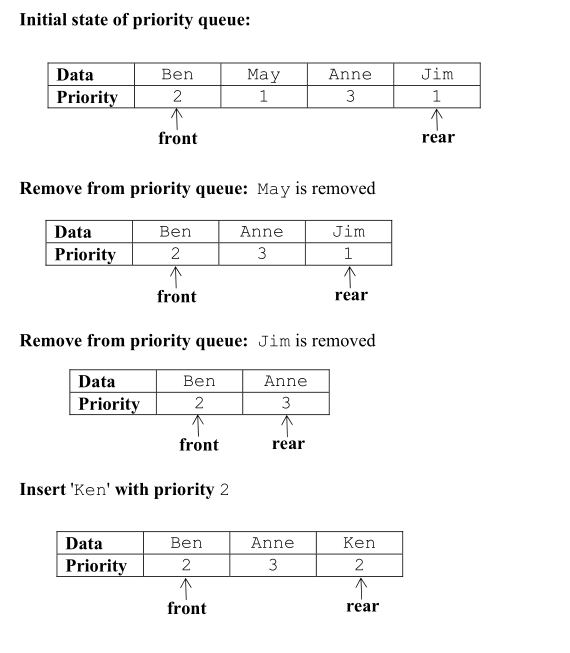
\includegraphics[width=0.5\paperwidth]{C:/Users/Admin/Desktop/Github/question_bank/LyX/static/img/9569-HCI-2021-P2-Q3-1}
\par\end{center}

A \textbf{priority queue} abstract data type (ADT) is to be implemented
as a linked list using object- oriented programming. Two classes \texttt{Node}
and \texttt{PQueue} have been identified.
\begin{center}
\begin{tabular}{|l|l|l|}
\hline 
\multicolumn{3}{|c|}{\texttt{Class: Node}}\tabularnewline
\hline 
\texttt{\hspace{0.01\columnwidth}}Identifier & \texttt{\hspace{0.01\columnwidth}}Data Type & \texttt{\hspace{0.05\columnwidth}}Description\tabularnewline
\hline 
\texttt{Data} & \texttt{STRING} & The node data\tabularnewline
\hline 
\texttt{Priority} & \texttt{INTEGER} & Indicates priority of node. Smaller value has higher priority\tabularnewline
\hline 
\texttt{Next} & \texttt{INTEGER} & Pointer to next node in queue.\tabularnewline
\hline 
\end{tabular}
\par\end{center}

\begin{center}
\begin{tabular}{|l|l|l|}
\hline 
\multicolumn{3}{|c|}{\texttt{Class: PQueue}}\tabularnewline
\hline 
\texttt{\hspace{0.01\columnwidth}}Identifier & \texttt{\hspace{0.01\columnwidth}}Data Type & \texttt{\hspace{0.05\columnwidth}}Description\tabularnewline
\hline 
\texttt{ThisPQueue} & \texttt{ARRAY{[}1:10{]} Of Node} & The priority queue data.\tabularnewline
\hline 
\texttt{Front} & \texttt{INTEGER} & Index for front node of queue.\tabularnewline
\hline 
\texttt{Rear} & \texttt{INTEGER} & Index for rear node of queue.\tabularnewline
\hline 
\texttt{NextFree} & \texttt{INTEGER} & Index for the next unused node.\tabularnewline
\hline 
\multirow{2}{*}{\texttt{Initialise()}} & \multirow{2}{*}{\texttt{PROCEDURE}} & - Set pointers to indicate all nodes are unused and linked. \tabularnewline
 &  & - Initialise values for \texttt{Front}, \texttt{Rear} and \texttt{NextFree}.\tabularnewline
\hline 
\multirow{2}{*}{\texttt{PQInsert(NewItem, Priority)}} & \multirow{2}{*}{\texttt{PROCEDURE}} & - Assign \texttt{NewItem} and \texttt{Priority} passed as parameters
to a node.\tabularnewline
 &  & - Insert the node to the rear of the priority queue.\tabularnewline
\hline 
\multirow{2}{*}{\texttt{PQDelete()}} & \multirow{2}{*}{\texttt{FUNCTION}} & - Remove a node of highest priority from the priority queue.\tabularnewline
 &  & - Return the \texttt{Data} attribute of the node that is removed.\tabularnewline
\hline 
\texttt{DisplayPQueue()} & \texttt{PROCEDURE} & Display the values of \texttt{Front}, \texttt{Rear}, \texttt{NextFree}
and the contents of \texttt{ThisPQueue} array in index order.\tabularnewline
\hline 
\end{tabular}
\par\end{center}

The diagram shows the linked list with: 
\begin{itemize}
\item the data items \texttt{'Ben'}, \texttt{'May'}, \texttt{'Anne'} and
\texttt{'Jim'} (inserted in that order) in the priority queue 
\item the unused nodes linked together 
\begin{center}
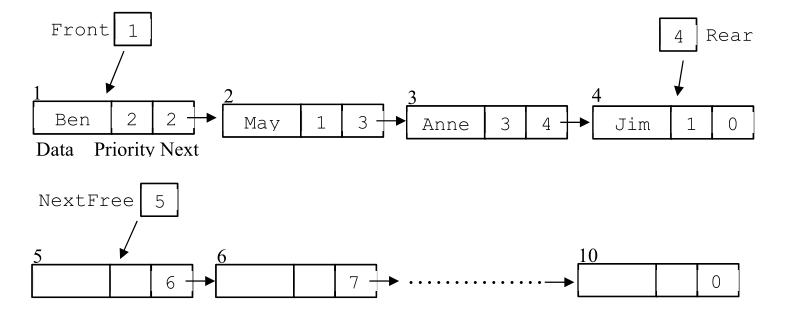
\includegraphics[width=0.5\paperwidth]{C:/Users/Admin/Desktop/Github/question_bank/LyX/static/img/9569-HCI-2021-P2-Q3-2}
\par\end{center}

\end{itemize}
For each of the sub-tasks, add a comment statement at the beginning
of the code using the hash symbol \textquoteleft \#\textquoteright ,
to indicate the sub-task the program code belongs to, for example: 
\noindent \begin{center}
\begin{tabular}{c|l|}
\cline{2-2} 
\multirow{2}{*}{\texttt{In{[}1{]}:}} & \texttt{\# Task 3.1}\tabularnewline
 & \texttt{Program Code}\tabularnewline
\cline{2-2} 
\multirow{2}{*}{\texttt{In{[}2{]}:}} & \texttt{\# Task 3.2}\tabularnewline
 & \texttt{Program Code}\tabularnewline
\cline{2-2} 
\multirow{2}{*}{\texttt{In{[}3{]}:}} & \texttt{\# Task 3.3}\tabularnewline
 & \texttt{Program Code}\tabularnewline
\cline{2-2} 
\multicolumn{1}{c}{} & \multicolumn{1}{l}{\texttt{Output:}}\tabularnewline
\end{tabular}
\par\end{center}

\subsubsection*{Task 3.1 }

Write program code for the classes \texttt{Node} and \texttt{PQueue},
including the \texttt{Initialise}, \texttt{PQInsert}, \texttt{PQDelete}
and \texttt{DisplayPQueue} methods. The code should follow the specification
given. \hfill{}{[}17{]}

\subsubsection*{Task 3.2 }

The program is to be tested. 

Write a main program to: 
\begin{itemize}
\item create a \texttt{PQueue} object 
\item read from file \texttt{PATIENTS.txt} all the data items with its priorities
into the priority queue by calling \texttt{PQInsert} method. 
\item output the priority queue by calling \texttt{DisplayPQueue} method.
\hfill{}{[}2{]}
\end{itemize}

\subsubsection*{Task 3.3 }

Write additional code in your main program to do the following in
order by calling the appropriate methods from \texttt{PQueue} class. 
\noindent \begin{center}
\begin{tabular}{|l|l|l|l|}
\hline 
No.  & Operation  & Data  & Priority\tabularnewline
\hline 
1  & Remove patient & \texttt{-} & \texttt{-}\tabularnewline
\hline 
2  & Remove patient  & \texttt{-} & \texttt{-}\tabularnewline
\hline 
3  & Add patient Carol & \texttt{Carol} & \texttt{4}\tabularnewline
\hline 
4  & Remove patient & \texttt{-} & \texttt{-}\tabularnewline
\hline 
5  & Remove patient & \texttt{-} & \texttt{-}\tabularnewline
\hline 
6  & Display priority queue  & \texttt{- } & \texttt{-}\tabularnewline
\hline 
\end{tabular}
\par\end{center}

Save your Jupiter Notebook for Task 3. \hfill{}{[}3{]}

{[}SPLIT\_HERE{]}
\item \textbf{{[}HCI/PRELIM/9569/2021/P2/Q4{]}}

Name your Jupyter Notebook as 

\texttt{TASK4\_<your name>\_<centre number>\_<index number>.ipynb }

The task is to write program code for a Tic-Tac-Toe-Tomek game for
two players. 

Tic-Tac-Toe-Tomek is a game played on a 4 x 4 square board. The board
starts empty, except that a single 'T' symbol may appear in one of
the 16 squares. There are two players: X and O. They take turns to
make moves, with X starting. In each move a player puts her symbol
in one of the empty squares. Player X's symbol is \texttt{'X'}, and
player O's symbol is \texttt{'O'}. 

After a player's move, if there is a row, column or a diagonal containing
4 of that player's symbols, or containing 3 of her symbols and the
\texttt{'T'} symbol, she wins and the game ends. Otherwise the game
continues with the other player's move. If all of the fields are filled
with symbols and nobody won, the game ends in a draw. 

Given the 4 x 4 board description containing \texttt{'X'}, \texttt{'O'},
\texttt{'T'} and \texttt{'.'} characters (where \texttt{'.'} represents
an empty square). The following examples show the various winning
positions. 
\begin{center}
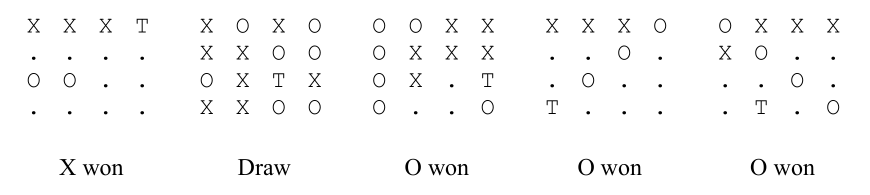
\includegraphics[width=0.5\paperwidth]{C:/Users/Admin/Desktop/Github/question_bank/LyX/static/img/9569-HCI-2021-P2-Q4}
\par\end{center}

For each of the sub-tasks, add a comment statement at the beginning
of the code using the hash symbol \textquoteleft \texttt{\#}\textquoteright ,
to indicate the sub-task the program code belongs to, for example: 
\noindent \begin{center}
\begin{tabular}{c|l|}
\cline{2-2} 
\multirow{2}{*}{\texttt{In{[}1{]}:}} & \texttt{\# Task 4.1}\tabularnewline
 & \texttt{Program Code}\tabularnewline
\cline{2-2} 
\multirow{2}{*}{\texttt{In{[}2{]}:}} & \texttt{\# Task 4.2}\tabularnewline
 & \texttt{Program Code}\tabularnewline
\cline{2-2} 
\multirow{2}{*}{\texttt{In{[}3{]}:}} & \texttt{\# Task 4.3}\tabularnewline
 & \texttt{Program Code}\tabularnewline
\cline{2-2} 
\texttt{In{[}4{]}:} & \texttt{\# Task 4.4}\tabularnewline
 & \texttt{Program Code}\tabularnewline
\cline{2-2} 
\texttt{In{[}5{]}:} & \texttt{\# Task 4.5}\tabularnewline
 & \texttt{Program Code}\tabularnewline
\cline{2-2} 
\multicolumn{1}{c}{} & \multicolumn{1}{l}{\texttt{Output:}}\tabularnewline
\end{tabular}
\par\end{center}

\subsubsection*{Task 4.1 }

Write program code to: 
\begin{itemize}
\item initialize the data structure to represent the 4 x 4 square board,
using the identifier \texttt{board} 
\item generate a pair of random numbers between 1 and 4 
\item place \texttt{'T'} at that random position on the board \hfill{}{[}3{]}
\end{itemize}

\subsubsection*{Task 4.2 }

Write a function \texttt{displayBoard} that will display the game
board clearly to the players. You should use the \texttt{board} as
a parameter in \texttt{displayBoard}. \hfill{}{[}2{]}

\subsubsection*{Task 4.3 }

Write a function \texttt{getPlayerMove} to get players to make their
move (by marking \texttt{'X'} or \texttt{'O'}) on the board. You should
include validation on player\textquoteright s input and check that
the space is not already occupied. Use \texttt{board} as a parameter.
You may include any other suitable parameters. \hfill{}{[}4{]}

\subsubsection*{Task 4.4 }

Write a function \texttt{checkWin} that checks all the conditions
for winning a game and returns \texttt{True} if a player has won the
game, otherwise returns \texttt{False}. Use \texttt{board} as a parameter.
You may include any other suitable parameters. \hfill{} {[}5{]}

\subsubsection*{Task 4.5 }

Write a \texttt{main} function that makes use of the identifiers and
functions from Task 4.1 to Task 4.4 and allows two players, X and
O, to play a game of Tic-Tac-Toe-Tomek. 

The \texttt{main} function should include the following: 
\begin{itemize}
\item display the initial game board with the single \texttt{'T}' displayed
in it 
\item start with player X to make the first move 
\item ensure players X and O take turns to make their move 
\item display the game board after every move made by a player 
\item check for winner 
\item display message on which player has won the game or whether the game
ends in a draw. \hfill{} {[}7{]}
\end{itemize}
Run your \texttt{main} function and produce outputs of \textbf{three}
games where player X wins one game, player O wins another game, and
a drawn game. 

Copy and paste all outputs in a text file as 

\texttt{TASK4\_5\_<your name>\_<centre number>\_<index number>.txt}
\hfill{} {[}3{]}

Save your Jupyter Notebook for Task 4. 

{[}SPLIT\_HERE{]}
\end{enumerate}
 
\end{document}
